\documentclass[]{beamer}
\usetheme[block=fill,progressbar=frametitle,numbering=none]{metropolis}
% Paquetes de la ams
\usepackage{amsmath,amsthm,amssymb,amsfonts}
% Codificacion UTF-8
\usepackage[utf8]{inputenc}
% Tablas e imagenes en espaniol
\usepackage[spanish,es-tabla]{babel}
% Mejores graficos
\usepackage{graphicx}
% tablas mas lindas
\usepackage{booktabs}
% Links a urls
\usepackage{url}
% Linkear referencias en pdfs
\usepackage{hyperref}
% Texto mas lindo para los pie de figura
\usepackage[margin=10pt,font=small,labelfont=bf, labelsep=endash]{caption}

% Citas
\usepackage[backend=biber,style=ieee]{biblatex}
\addbibresource{biblio.bib}

% Codigo
\usepackage{listings}

% Dir tree
\usepackage{dirtree}

% Pagina en blanco cuando ha
\usepackage{emptypage}

\definecolor{A11}{HTML}{B2DF8A}
\definecolor{A12}{HTML}{33A02C}
\definecolor{A23}{HTML}{FDBF6F}
\definecolor{A24}{HTML}{FF7F00}
\definecolor{B15}{HTML}{FB9A99}
\definecolor{B16}{HTML}{E31A1C}
\definecolor{B27}{HTML}{A6CEE3}
\definecolor{B28}{HTML}{1F78B4}

% Ejemplos, observaciones y teorema
\theoremstyle{definition}
\newtheorem{exa}{Ejemplo}[section]
\newtheorem*{obs}{Observación}
\newtheorem{que}{Pregunta}[section]
\newtheorem{dex}{Definicion}[section]

\author{Francisco Nemiña}
\title{Nivel 2: herramientas de teledetección cuantitativa}
\subtitle{El espectro electromagnético}
\institute{Unidad de Educación y Formación Masiva \\ Comisión Nacional de Actividades Espaciales}
\date{}
\graphicspath{{./figs/}}

\begin{document}

\maketitle


\begin{frame}{Table of contents}
  \setbeamertemplate{section in toc}[sections numbered]
  \tableofcontents[hideallsubsections]
\end{frame}

\section{Radiación}
\label{sec:radiacion}
\begin{frame}{Energía}
  \begin{block}{Definicíon}
    Energía es la capacidad de hacer trabajo... \pause ponele.
  \end{block}
\end{frame}
%--- Next Frame ---%

\begin{frame}{Energía}
  Es mas fácil hablar de las formas de propagación
  \begin{figure}
    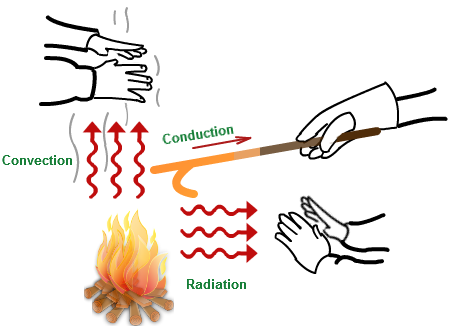
\includegraphics[width=0.6\textwidth]{types-of-heat-transfer.png}
    \caption{Formas de transferencia de energía calor.}
  \end{figure}
\end{frame}


\begin{frame}{Energía electromagnética}
  \begin{figure}
    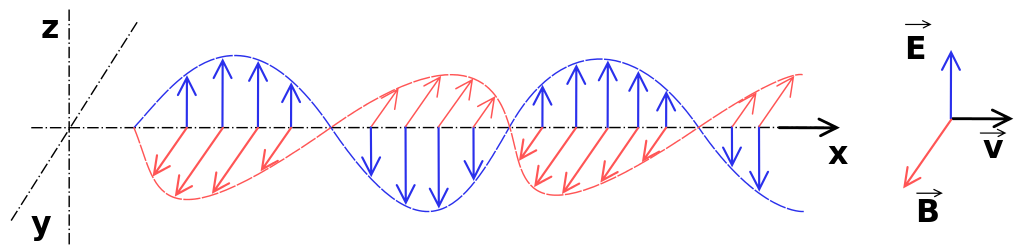
\includegraphics[width=0.6\textwidth]{Onde_electromagnetique.png}
    \caption{De las 3, nos vas a interesar la radiación. En particular la radiación electromagnética.\footfullcite{wiki:onda}}
  \end{figure}
\end{frame}
%--- Next Frame ---%

\begin{frame}{Onda electromagnética}
  \begin{block}{Definición}
    La longitud de onda es la distancia entre dos máximos.
  \end{block}\pause
  \begin{block}{Definición}
    La frecuencia es la cantidad de oscilaciones que realiza la onda por unidad de tiempo.
  \end{block}\pause
  \begin{block}{Definición}
    La amplitud es el máximo valor posible que toma la onda.
  \end{block}
\end{frame}
%--- Next Frame ---%

\begin{frame}{Clasificación}
  \begin{figure}
    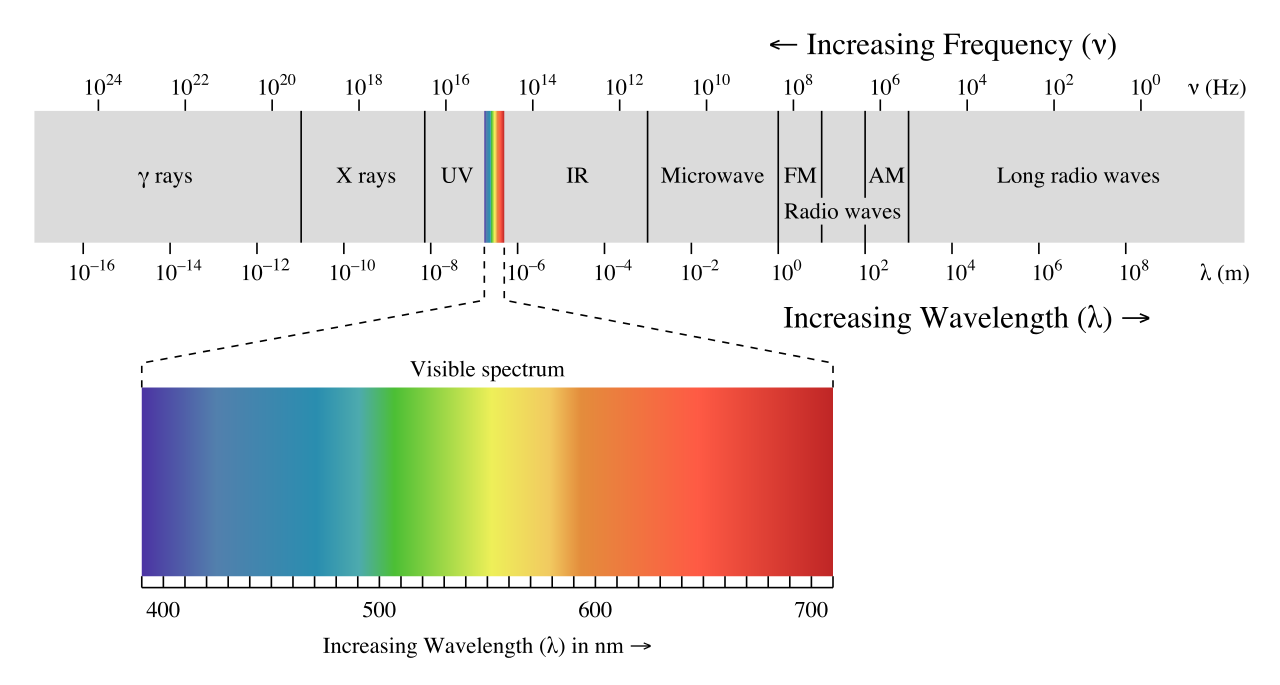
\includegraphics[width=0.8\textwidth]{espectrum.png}
    \caption{Las ondas electromagnéticas se pueden clasificar en función de su longitud de onda en el espectro electromagnético. \footfullcite{spectrum}}
  \end{figure}
\end{frame}
%--- Next Frame ---%

\end{document}
